\chapter{РЕАЛИЗАЦИЯ ФРЕЙМВОРКА}
\label{ch:РЕАЛИЗАЦИЯ ФРЕЙМВОРКА}

В этой главе дается описание разработки фреймворка с предоставлением деталей реализации описанной ранее концепции на базе выбранного стека технологий. На основе изложенного ранее рабочего процесса фреймворка были реализованы отдельные модули, подробное описание каждого из них представлено в следующих разделах. Первые разделы описывают обработку и аппроксимацию входных данных траектории. В последующих разделах представлены детали реализации решения задач кластеризации, моделирования кластеров и классификации входных траекторий. По причине того что не было найдено подходящих готовых реализаций для выбранных алгоритмов, все реализации алгоритмов, кроме полиномиальной регрессии и решения полиномиальных уравнений, были написаны с нуля и представлены в Приложениях.

\section{Используемые технологии}

Для реализации фреймворка был выбран язык программирования Java с сопутствующими библиотеками и Apache Maven в качестве инструмента для автоматизации сборки для проектов Java следующих версий:

\begin{itemize}
	\item Java - 11 OpenJDK
	\item Apache Maven - 3.6.3
	\item Commons Math: The Apache Commons Mathematics Library - 3.4.1
	\item Java AWT, Javax Swing 
\end{itemize}

Java используется как основной язык программирования. Библиотека Commons Math library была выбрана для реализации аппроксимации траекторий, поскольку она предлагает реализацию для таких классов, как $PolynomialFunction$ и $PolynomialSolver$. 

Java AWT (Abstract Window Toolkit) представляет собой ИПП (Интерфейс прикладного программирования, API) для реализации ГПИ (Графический Пользовательский Интерфейс, GUI) в Java приложениях и поставляется как часть Java JDK начиная с версии OpenJDK 7. В данной работе Java AWT будет использоваться преимущественно для создания и манипуляции объектами $BufferedImage$ для визуализации исходных изображений с камер и отображения траекторий на них.

Java Swing, так же как и Java AWT, является инструментальной библиотекой, созданной для тех же целей предоставления ГПИ приложениям, написанным на Java, и реализации возможности написания приложений, основанных на применении окон (оконных приложений). Однако Swing является более новой и продвинутой библиотекой, поддерживающей более сложные, усовершенствованные ГПИ-компоненты, нежели Java AWT. В текущей работе Swing используется для создания окон для визуализации изображений с исходными траекториями, результатами аппроксимации и кластеризации.

\section{Работа со входными данными}
\subsection{Описание входных данных}

Согласно исследованию, проведенному Министерством транспорта США на основе данных Системы отчетов об анализе смертности (Fatality Analysis Reporting System, FARS) и Национальной системы отбора проб автомобилей (National Automotive Sampling System), почти 40 процентов всех зарегистрированных в 2008 году аварий произошли на перекрестках \cite{inproceedings:10_cfi}. Следовательно, в настоящее время анализ транспортной активности на перекрестках на перекерстках дорог имеет большое значение в контексте безопасности, и выявление небезопасных транспортных траекторий, нарушающих ПДД, может быть одним из шагов на пути к улучшению статистики.

В представленной работе видео с камер слежения используется для обучения и тестирования системы. Тестовые видео получены с помощью ИТС, реализованных и установленных на четырех перекрестках в г. Казань:

\begin{enumerate}
	\item Перекресток улиц Право-Булачная - Пушкина, $1.txt$ (рис. \ref{fig:is_1}).
	\item Перекресток улиц Несмелова - Кировская Дамба, $2.txt$ (рис. \ref{fig:is_2}).
	\item Перекресток улиц Московская - Галиаскара Камала, $3.txt$ (рис. \ref{fig:is_3}).
	\item Перекресток улиц Московская - Парижской Коммуны, $4.txt$ (рис. \ref{fig:is_4}).
\end{enumerate}

Каждый перекресток представляет собой четырехстороннее пересечение дорог, оборудованное одной регистрирующей камерой. Примеры изображений с установленных видеокамер представлены на рис. \ref{fig:is_all}.

\begin{figure}[!htb]
	\centering
	\begin{subfigure}[!htb]{0.48\textwidth}
		\centering{}
		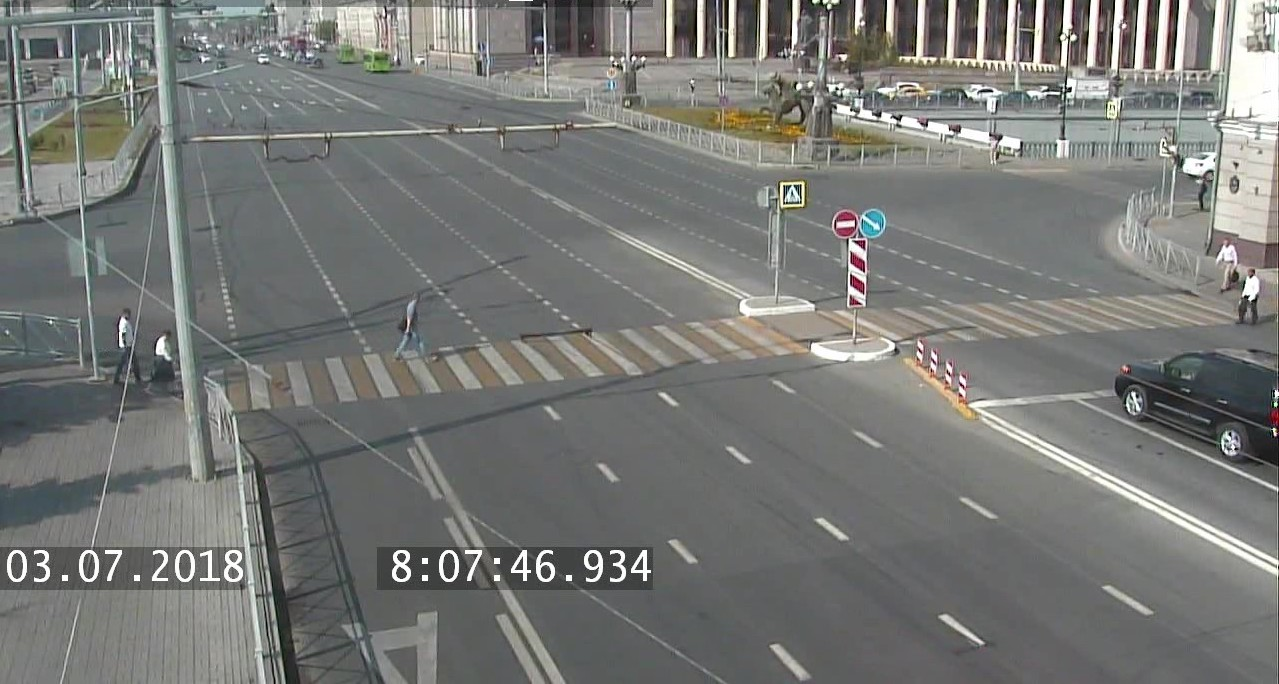
\includegraphics[width=\textwidth]{images/is-1.jpg}
		\caption{$1.txt$}
		\label{fig:is_1}
	\end{subfigure}
	\hfill
	\begin{subfigure}[!htb]{0.48\textwidth}
		\centering{}
		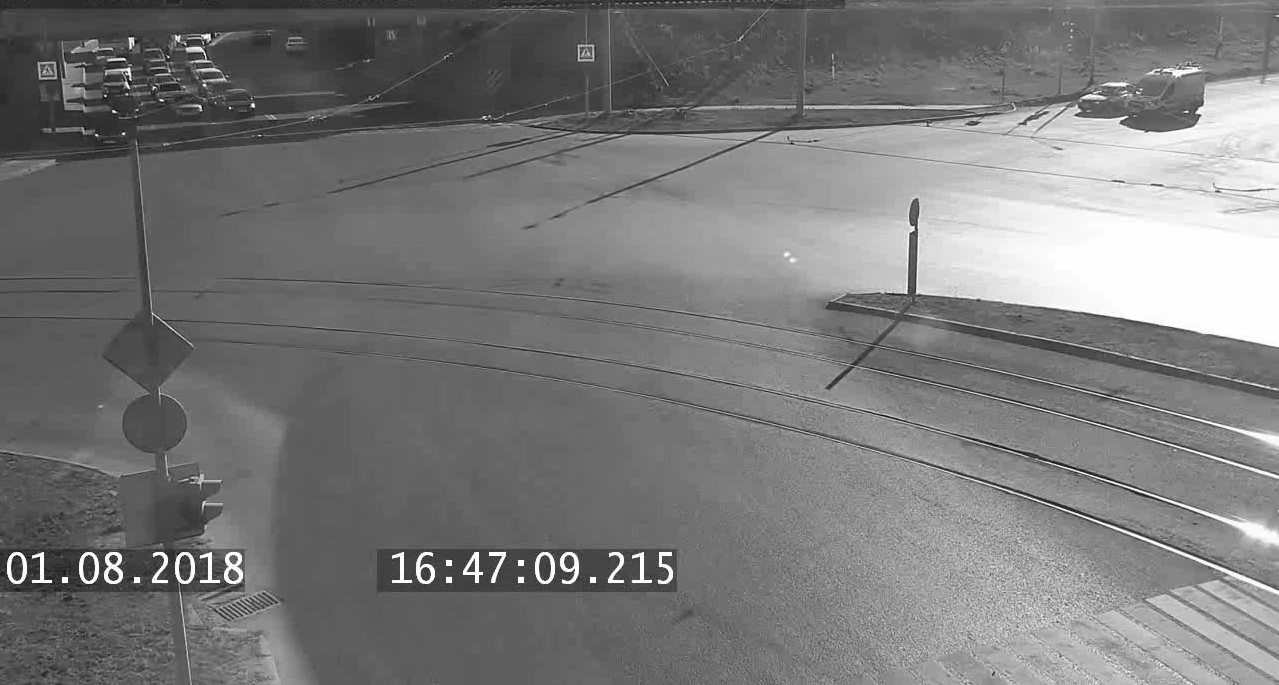
\includegraphics[width=\textwidth]{images/is-2.jpg}
		\caption{$3.txt$}
		\label{fig:is_2}
	\end{subfigure}
	\hfill
	\begin{subfigure}[!htb]{0.48\textwidth}
		\centering{}
		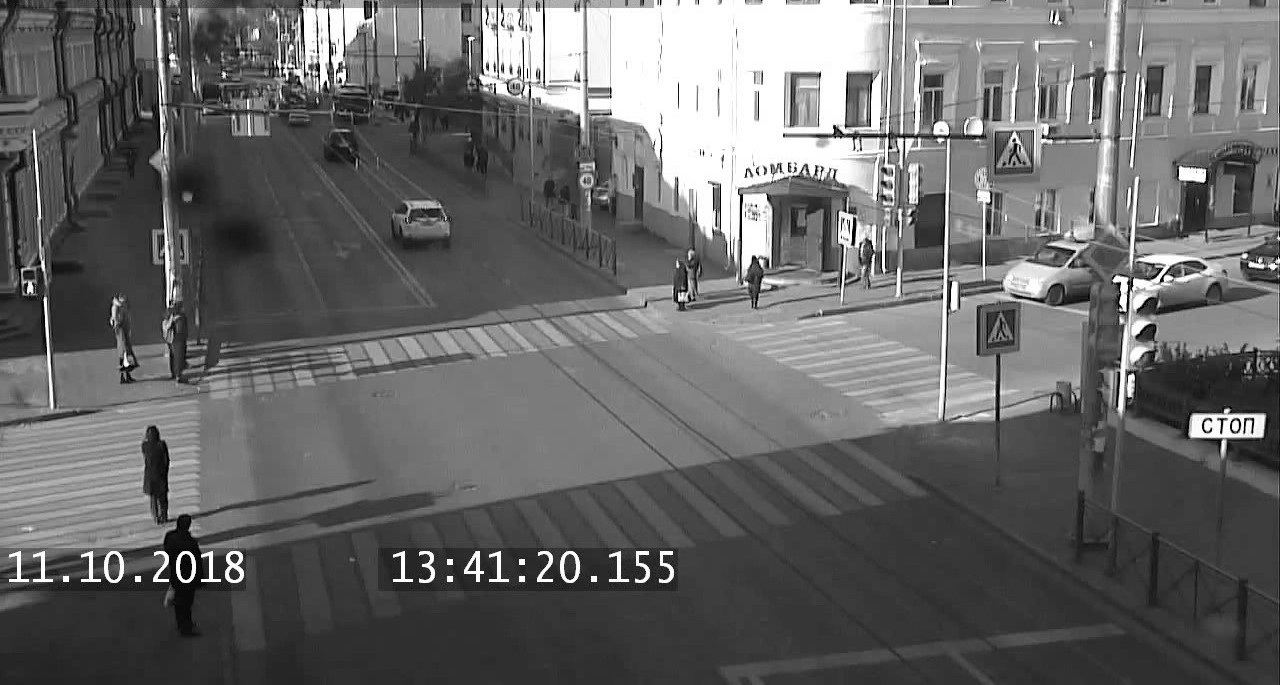
\includegraphics[width=\textwidth]{images/is-3.jpg}
		\caption{$4.txt$}
		\label{fig:is_3}
	\end{subfigure}
	\hfill
	\begin{subfigure}[!htb]{0.48\textwidth}
		\centering{}
		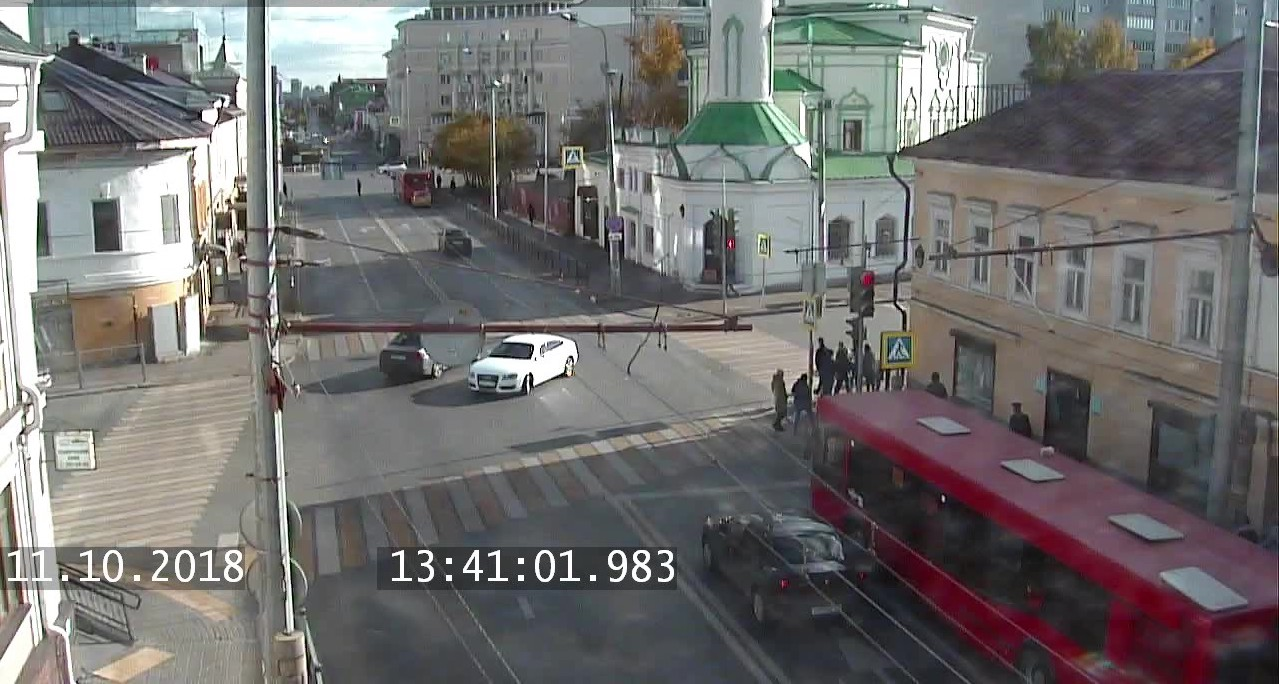
\includegraphics[width=\textwidth]{images/is-4.jpg}
		\caption{$4.txt$}
		\label{fig:is_4}
	\end{subfigure}
	\caption{Примеры изображений с видеокамер на перекрестках 1-4}
	\label{fig:is_all}
\end{figure}

Файлы с входными данными содержат 624, 211, 231, 237 траекторий ТС для каждого из указанных перекрестков соответственно.

Под аномальной траекторией подразумевается траектория движения ТС через перекресток, которая значительно отличается от большинства известных, нормальных траекторий. Например, в случае, когда на перекрестке запрещен поворот направо с крайней левой полосы движения, такое поведение будет неизвестно системе. В случае появления такой траектории она будет признана системой аномальной.

\begin{figure}[!htb]
	\centering{}
	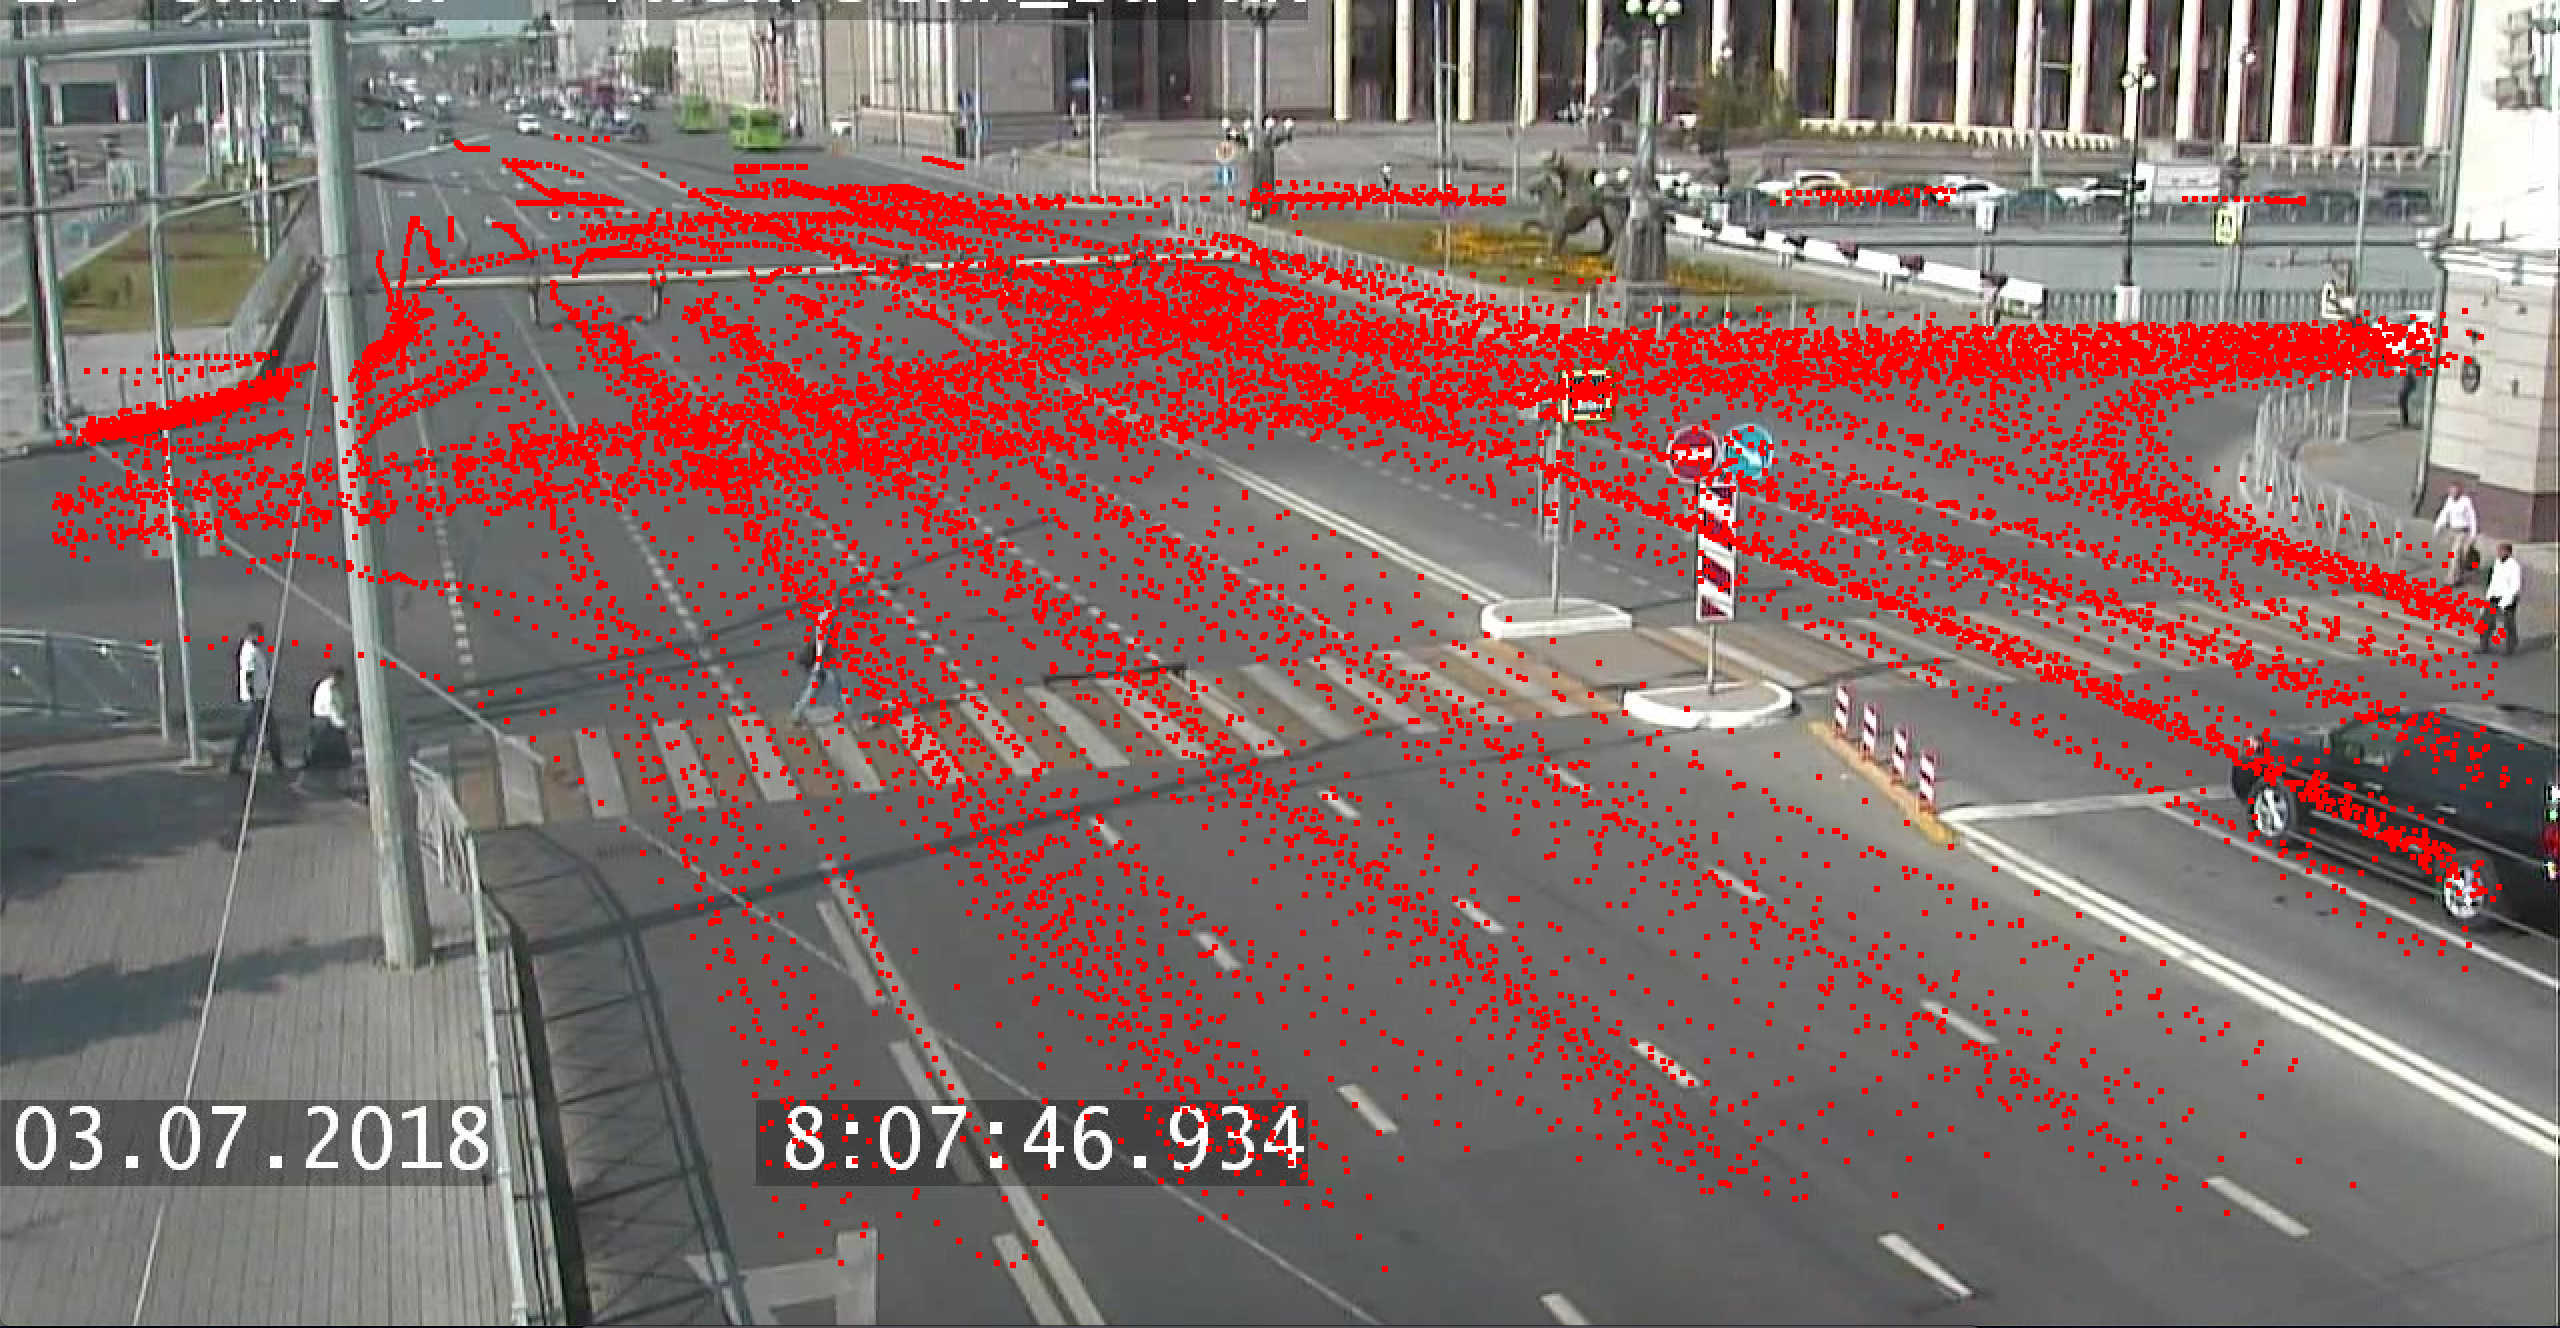
\includegraphics[width=0.8\textwidth]{images/tr-p.png}
	\caption{Пример работы системы слежения на данных с первого перекрестка}
	\label{fig:tr_p}
\end{figure}

\subsection{Структура файла входных данных}

Система отслеживания, как было описано ранее, обрабатывает видео с камер слежения и подготавливает его для дальнейшего анализа: преобразует видеопоток в набор векторов с точками отслеживания (далее точки траектории) на изображениях (рис. \ref{fig:tr_p}).

Файлы входных данных имеют следующую структуру:

\begin{equation} \label{eq:input_str}
[[[(x_1^1, y_1^1), ..., (x_1^n, y_1^n)], [t_1, ... t_n]], [[(x_2^1, y_2^1), ..., (x_2^m, y_2^m)], [t_1, ... t_m]], ...]
\end{equation}

Как видно из структуры файла входных данных, каждая траектория представлена двухэлементным массивом, где первый массив хранит координаты в виде массива пар $(x_i^j, y_i^j)$, а второй массив содержит временные метки для каждой пространственной точки в соответствующем порядке $(t_i)$. Извлеченные координаты $x$ и $y$ соответствуют пикселям на входных изображениях. В формуле \ref{eq:input_str} нижний индекс пространственных координат указывает на порядковый номер траектории, а верхний индекс представляет собой порядковый номер точки отслеживания. Внешний массив является массивом траекторий.

\subsection{Обработка входных данных}

Поскольку выбранный алгоритм ожидает получить траектории в виде многомерных векторов, исходные входные данные необходимо преобразовать к подходящему формату. Для этих целей был реализован пользовательский парсер, принимающий текстовый файл ``txt'' с траекториями в указанном ранее формате в качестве входных данных и в результате возвращающий список объектов $Trajectory$. Объект $Trajectory$ состоит из нескольких объектов $TrajectoryPoint$ со следующими атрибутами: \textit{x}-координата, \textit{y}-координата, время \textit{t}. Исходный код метода синтаксического анализа приведен в Приложении А.

Входные данные содержат траектории различной длины и с различным пройденным расстоянием. Однако из-за неточности и ошибок в системе слежения некоторые траектории выглядят неправдоподобно и не имеют смысла. Одна из возможных причин этого - пропавший отслеживаемый объект или потеря системой слежения местоположения объекта. В отличие от случая потерянного местоположения, когда пропущенное местоположение может быть найдено с использованием моделей аппроксимации и регрессии, потерянный объект отслеживания не может быть впоследствии исправлен. По этой причине, чтобы улучшить качество результатов, было решено отфильтровать входные траектории и игнорировать короткие траектории с малым пройденным расстоянием, где пройденное расстояние рассчитывается как евклидово расстояние между первой и последней точками траектории. Для фильтрации параметров использовались следующие значения: $minLength = 10\ (trajectory \ points)$, $minTotalDist = 80 \ (pixels)$. Результаты фильтрации с отображением удаленных и сохраненных траекторий показаны на рис. \ref{fig:traj_filter}.

\begin{figure}
	\centering
	\begin{subfigure}[b]{0.48\textwidth}
		\centering{}
		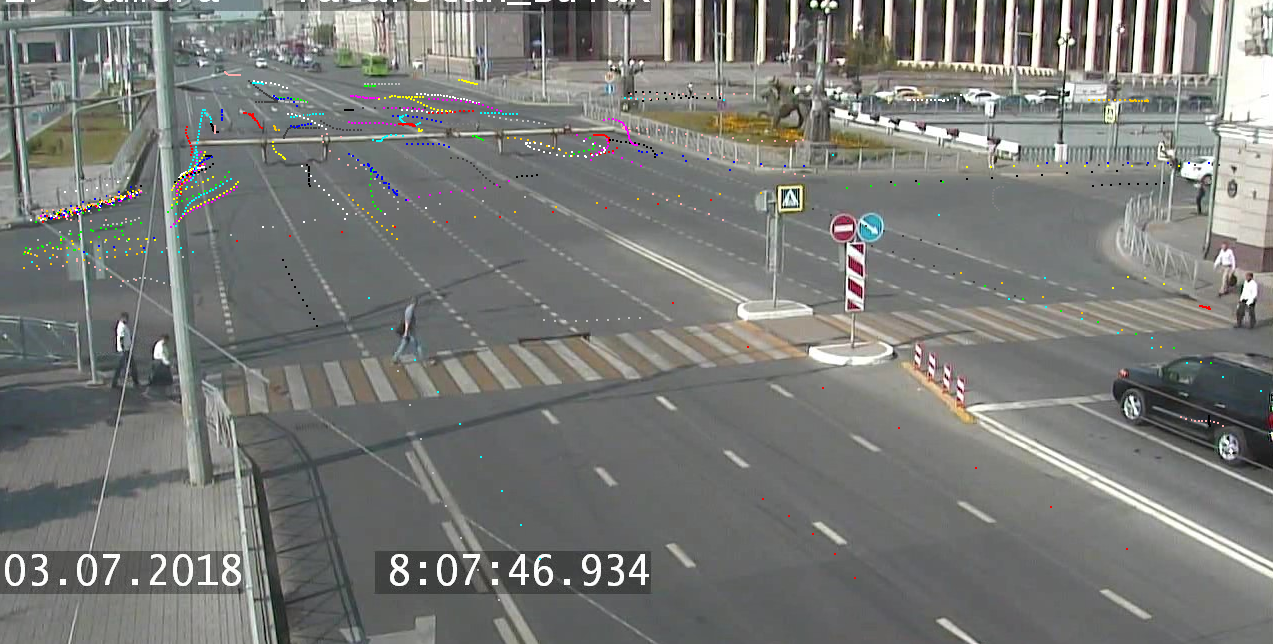
\includegraphics[width=\textwidth]{images/traj-filter-out.png}
		\caption{игнорируемые траектории}
		\label{fig:traj_filter_out}
	\end{subfigure}
	\hfill
	\begin{subfigure}[b]{0.48\textwidth}
		\centering{}
		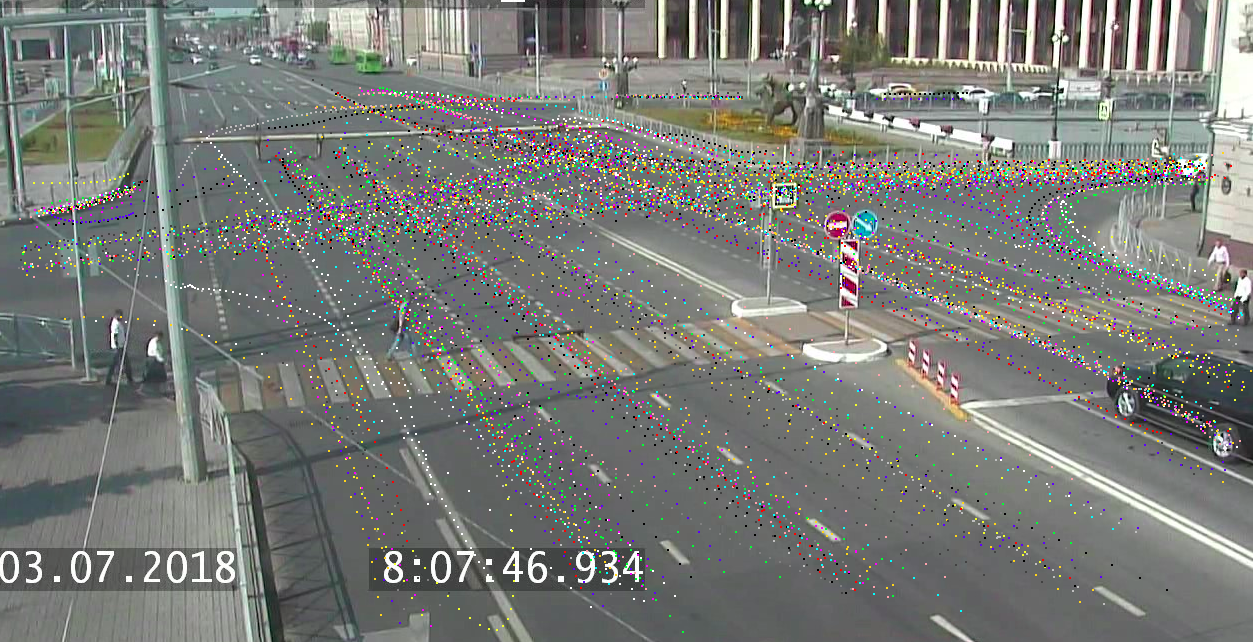
\includegraphics[width=\textwidth]{images/traj-filter-keep.png}
		\caption{оставленные траектории}
		\label{fig:traj_filter_keep}
	\end{subfigure}
	\caption{Результаты фильтрации траекторий на примере данных с первого перекрестка}
	\label{fig:traj_filter}
\end{figure}

Как уже упоминалось ранее, текущая работа сфокусирована на задаче выявления двух типов нарушений: пространственных и пространственно-временных. Для выявления аномалий первой группы достаточно проанализировать пространственную информацию о траекториях. Обнаружение аномалий второй категории, которая формируется из траекторий ТС, движущихся с аномально низкой или высокой скоростью, требует учета временной информации вместе с пространственной. По этой причине средняя постоянная скорость $\upsilon$ рассчитывается для каждой из входных траекторий $T$ в конце этапа парсинга данных как (\ref{eq:avg_speed}):

\begin{equation} \label{eq:avg_speed}
\upsilon_{avg}(T) = \frac{distance_{total}} {time_{total}},
\end{equation}

где $distance_{total}$ - итоговое пройденное расстояние между первой и последней точками траектории, а $time_{total}$ - прошедшее время. Общее расстояние может быть вычислено как сумма евклидовых расстояний между точками траектории на соседних кадрах. Поскольку известно, что кадры сняты с межкадровым интервалом 0,01 секунды, вычисление скорости может быть реализовано следующим образом (лист. \ref{lst:speed-calc}):

\lstset{style=code-style-java}
\lstinputlisting[caption={Подсчет скорости ТС}, label={lst:speed-calc}] {listings/calcSpeed.java}

\subsection{Аппроксимация траекторий с использованием Полиномиальной Регрессии}

Как обсуждалось ранее, полиномиальная регрессия будет использоваться для аппроксимации исходных траекторий. Были использованы готовые реализации классов-сущностей полинома\footnote{Реализация полинома \url{https://javadoc.io/doc/org.apache.commons/commons-math3/3.4.1/org/apache/commons/math3/analysis/polynomials/PolynomialFunction.html}} (необходим для дальнейшего анализа уравнений аппроксимации и поиска ключевых точек) и метода решения полиномиальных уравнений\footnote{Реализация метода решения полиномиальных функций \url{https://www.javadoc.io/doc/org.apache.commons/commons-math3/3.4.1/org/apache/commons/math3/analysis/solvers/LaguerreSolver.html}} из библиотеки Apache Commons Math 3.4.1. Для выполнения полиномиальной регрессии\footnote{Реализация полиномиальной регрессии \url{https://algs4.cs.princeton.edu/14analysis/PolynomialRegression.java}} была выбрана реализация, предоставленная авторами Р. Седжвиком и К. Уэйном для языка программирования Java \cite{online:polynomial_impl}. Все готовые к использованию реализации были пользовательскими вспомогательными методами.

Класс $PolynomialRegression$ принимает в качестве входных данных ожидаемую степень аппроксимирующего полинома ($d$) и два массива данных из N точек, состоящих из действительных чисел: массив независимых переменных ($double[]\ t$), данные о времени в данном случае, и массив зависимых переменных ($double[]\ x$, $double[]\ y$), пространственные $x$- или $y$-координаты. Затем он выполняет полиномиальную регрессию для входного набора из N точек данных $(t_i, x_i)$ или $(t_i, y_i)$ и пытается подобрать многочлен $x = \beta_0 + \beta_1 t + \beta_2 t^2 + \ldots \beta_d t^d$, где $\beta_i$ - коэффициенты регрессии, минимизирующие сумму квадратов ошибок модели полиномиальной регрессии. Поиск наилучшего решения для полиномиальных параметров основан на методе наименьших квадратов \cite{article:behav_form_extr}.

Для достижения лучшей аппроксимации оценка результатов полиномиальной регрессии выполнялась с использованием коэффициента детерминации, обозначаемого как $R^2$ (также известного как $R$-$squared$, $R$-$квадрат$ оценка, \textit{коэффициент регрессии Пирсона}) \cite{inbook:stats}. $R^2$ измеряет долю дисперсии зависимой переменной, которая может быть объяснена регрессионной моделью с заданными параметрами и является предсказуемой из независимой (объясняющей) переменной, и вычисляется следующим образом:

\begin{equation}\label{eq:r_sq}
	R^2 = 1 - \frac{SSE}{TSS} = 1 - \frac{\sum{(y_i - \hat{y_i})^2}}{\sum{(y_i - \overline{y})^2}}
\end{equation}

где $SSE$ (Sum of Squares due to Error, сумма квадратов остатков, или ошибок, регрессии) рассчитывается как сумма квадратов разностей между фактическими значениями $y_i$ и прогнозируемыми (расчетными) значениями зависимых переменных $\hat{y_i}$, и $TSS$ (Total Sum of Squares, общая сумма квадратов) рассчитывается как сумма квадратов отклонений фактического значения $y_i$ от среднего значения $\overline{y}$.

Коэффициент $R^2$ может принимать значения между [0, 1], где близкое к 1 значение указывает на то, что существует сильная зависимость меду выбранными параметрами и модель (в данном случае полиномиальное уравнение) отлично предсказывает данные \cite{online:reg_r_interpr}. Модели со значением коэффициента выше 0,8 принято считать адекватными, значение 1 свидетельствует о наличии функциональной зависимости между переменными.

В этой работе полиномиальная регрессия была выполнена для всех исходных траекторий (Приложение B). Полученные регрессионные модели сравнивались по показателям $R^2$, результаты анализировались относительно формы и скорости траекторий. Демонстрация, сравнение и обсуждение полученных результатов представлены в следующей главе.

\subsection{Выбор ключевых точек в аппроксимированных траекториях}

Главной целью и причиной использования аппроксимированных траекторий вместо исходных для дальнейшего анализа было уменьшение сложности подсчета LCSS метрики. По этой причине длина траекторий должна быть уменьшена путем выбора нескольких ключевых репрезентативных точек из аппроксимированных траекторий путем анализа полиномов аппроксимации.

Из математики известно, что критическими точкам полинома $f(t)$ являются точки, где полиномиальная функция не дифференцируема или производная в этой точке равна нулю (стационарные точки). Стационарные точки, включая локальные минимумы и максимумы, восходящие и нисходящие точки перегиба можно найти путем анализа производных функции. Стационарные точки являются решениями уравнения, в котором первая производная функции приравнена нулю: $f'(t) = 0$. Точки перегиба могут быть найдены путем дальнейшего анализа второй производной: они соответствуют решениям уравнения $f''(t) = 0$. Для решения полиномиальных уравнений использовались готовые релизации метдов решения полиномиальных уравнений из библиотеки Apache Commons Math: $LaguerreSolver$, $BisectionSolver$ со следующими входными параметрами:

\begin{itemize}
	\item $maxItem = 30000$ -- задает максимально допустимое количество итераций в ходе поиска решения полиномиального уравнения,
	\item $min = firstTimePoint$ -- определяет нижнюю границу допустимых значений решения;
	\item $max = lastTimePoint$ -- определяет верхнюю границу допустимых значений решения;
	\item $startValue = min + 1$ -- задает начальную точку для метода решения уравнения, чтобы начать поиск решения.
\end{itemize}

Программа решения уравнений вызывалась для полиномиальных функций, полученных как первая и вторая производные, взятые из полиномов для $X$- и $Y$-координат. Вызов метода решения приведен в лист. \ref{lst:solver-init}:

\lstinputlisting[caption={Вызов метода решения полиномиальных уравнений}, label={lst:solver-init}] {listings/initSolver.java}

Решения, найденные двумя методами, объединяются: остаются только точки, относящиеся к разным точкам времени.

В случае анализа траекторий точки перегиба очень значимы и репрезентативны, поскольку они несут важную информацию о форме траектории: ключевые точки обозначают места основных поворотов или изменения траектории.

Однако критические точки не всегда могут быть найдены из-за вычислительных ограничений полиномиальных функций высокого порядка. Следовательно, критических точек, идентифицированных таким образом, недостаточно, чтобы полностью описать поведение исходной траектории и использовать для дальнейшего анализа, поскольку они не предоставляют всей информации о границах формы траектории и не всегда могут отобразить все повороты. По этой причине было решено добавить граничные для траектории ключевые точки, взяв отдельно минимальные и максимальные координаты $X$ и $Y$ и вычислив соответствующие точки траектории с использованием соответствующей регрессионной модели (лист. \ref{lst:key-borders-calc}).

\lstinputlisting[caption={Вычисление граничных ключевых точек траектории}, label={lst:key-borders-calc}] {listings/calcKeyBorders.java}

Результаты аппроксимации полиномиальной регрессией и вычисления ключевых точек представлены на рисунке \ref{fig:regr-kp}. Точки траектории, относящиеся к исходным данным траектории, изображены с использованием красного цвета, тогда как синие точки траектории соответствуют точкам, полученным с использованием функций полиномиального приближения для тех же временных точек. Ключевые точки каждой траектории выделены жирными синими квадратными точками. Видно, что функция аппроксимации близка к исходной функции траектории, для некоторых траекторий приближение дает те же координаты, что и в исходных данных (для траекторий с полиномами аппроксимации, имеющими $R^2 \approx 1.0$). Также можно заметить, что ключевые точки точно придерживаются линии аппроксимации и правильно описывают траекторию, следовательно, они могут использоваться вместо исходных точек траектории для упрощения дальнейшего анализа траекторий.

\begin{figure}[!htb]
	\centering
	\begin{subfigure}[!htb]{0.68\textwidth}
		\centering{}
		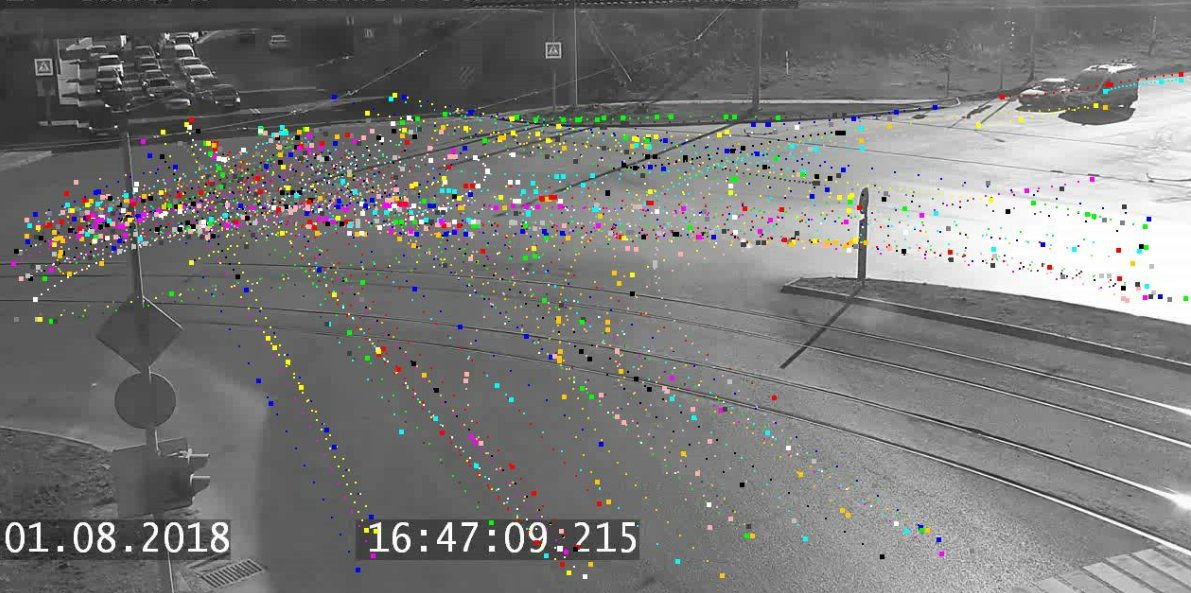
\includegraphics[width=\textwidth]{images/regr_kp_full.png}
		\caption{множество всех исходных траекторий $2.txt$}
	\end{subfigure}
	\hfill
	\begin{subfigure}[!htb]{0.3\textwidth}
		\centering{}
		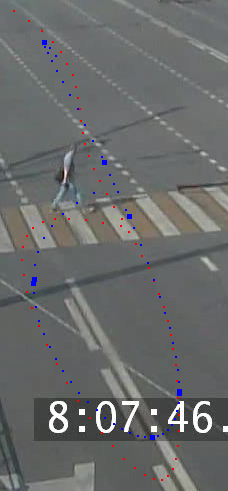
\includegraphics[width=\textwidth]{images/regr_kp_loop.png}
		\caption{траектория-петля $1.txt$}
	\end{subfigure}
	\hfill
	\begin{subfigure}[!htb]{0.3\textwidth}
		\centering{}
		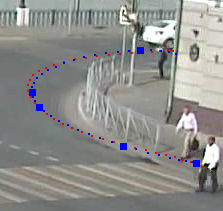
\includegraphics[width=\textwidth]{images/regr_kp_turn.png}
		\caption{траектория с поворотом $1.txt$}
	\end{subfigure}
	\hfill
	\begin{subfigure}[!htb]{0.3\textwidth}
		\centering{}
		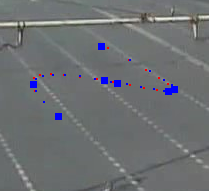
\includegraphics[width=\textwidth]{images/regr_kp_complex.png}
		\caption{траектория сложной формы $1.txt$}
	\end{subfigure}
	\hfill
	\begin{subfigure}[!htb]{0.3\textwidth}
		\centering{}
		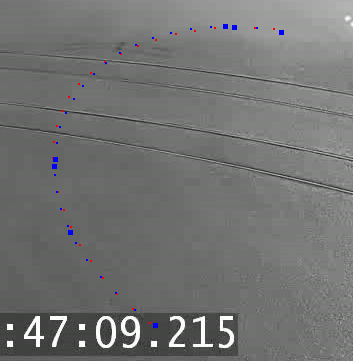
\includegraphics[width=\textwidth]{images/regr_kp_curve_2.png}
		\caption{изогнутая траектория $2.txt$}
	\end{subfigure}
	\hfill
	\begin{subfigure}[!htb]{0.3\textwidth}
		\centering{}
		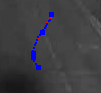
\includegraphics[width=\textwidth]{images/regr_kp_complex_3.png}
		\caption{траектория сложной формы $3.txt$}
	\end{subfigure}
	\hfill
	\begin{subfigure}[!htb]{0.3\textwidth}
		\centering{}
		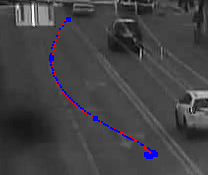
\includegraphics[width=\textwidth]{images/regr_kp_curve_3.png}
		\caption{изогнутая траектория $3.txt$}
	\end{subfigure}
	\hfill
	\begin{subfigure}[!htb]{0.3\textwidth}
		\centering{}
		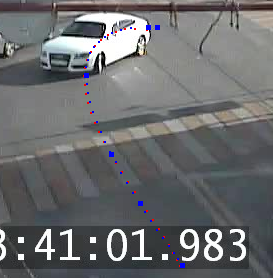
\includegraphics[width=\textwidth]{images/regr_kp_curve_4.png}
		\caption{траектория-поворот $4.txt$}
	\end{subfigure}

	\caption{Результаты полиномиальной регрессии с обозначением ключевых точек}
	\label{fig:regr-kp}
\end{figure}

\section{Анализ траекторий}
\subsection{Вычисление метрики схожести траекторий}

Как упоминалось ранее, LCSS метрика будет использоваться в качестве метрики для измерения сходства между траекториями. Следовательно, расстояние LCSS (метрика различия) будет рассчитываться на основе метрики сходства LCSS в соответствии с вышеупомянутыми формулами. Стоит отметить, что LCSS метрика является симметричной и для пары траекторий может быть вычислена только один раз \cite{inproceedings:28_lcss_dsmt}.

Несмотря на то что реализация LCSS метрики присутствует в пакете R \cite{online:r_lcss}, представленная реализация не позволяет использование динамических, адаптивных параметров $\delta$ и $\varepsilon$. По этой причине в рамках реализации фреймворка была написан пользовательская реализация метода подсчета LCSS метрики, представленный в лист. \ref{lst:lcss-calc}.

\lstinputlisting[caption={Вычисление LCSS}, label={lst:lcss-calc}] {listings/calcLCSS.java}

\subsection{Кластеризация}

Поскольку не было найдено подходящей реализации иерархической кластеризации для траекторий с использованием расстояния LCSS и возможностью обрабатывать адаптивные значения параметров, кластеризация, а также вычисление метрики LCSS, были написаны с нуля. Реализация была написана на основе алгоритма \ref{algo:ahc-descr}, представленного выше, в общих чертах описывающего алгоритм. Исходный код кластеризации приведен в Приложении С.

Кластеризация выполняется итеративно методом последовательного объединения двух ближайших кластеров в один с последующим пересчетом матрицы подобия (близости) кластеров. Метод кластеризации принимает в качестве входных данных параметр $OUTPUT\_CLUSTERS\_COUNT$, который определяет ожидаемое итоговое количество кластеров. Если полученное значение пустое ($null$), оно будет рассматриваться как 1, и кластеризация будет выполняться до тех пор, пока все кластеры не будут объединены в один в соответствии с базовым алгоритмом агломеративной иерархической кластеризации, или пока дальнейшее объединение кластеров будет невозможно.

\subsubsection{Валидация кластеров}

Как было описано ранее, валидация кластеров будет проводиться с ипользованием индекса Данна (DI). В лист. \ref{lst:di-calc} представлена реализация подсчета DI значения для итоговых кластеров.

\lstinputlisting[caption={Вычисление DI}, label={lst:di-calc}] {listings/diCalc.java}

Как видно из представленного листинга кода, сначала считается минимальная дистанция между всеми парами кластеров ($minDist$), затем выяисляется максимальный диаметр среди диаметров всех кластеров ($maxDiam$). Поскольку реализация основана на предположении, что траектории в кластерах появляются в порядке упорядочивания идентификаторов по возрастанию и внутренний цикл начинается с индекса, на 1 большего внешнего индекса кластера или траектории, перед подсчетами траектории кластеров будут упорядочены для упрощения дальнейших расчетов.

\subsection{Моделирование кластеров}

Clusters modeling implementation